\documentclass[10pt]{article}

% correct bad hyphenation here
\hyphenation{op-tical networks semi-conduc-tor}

% Initialise AMS maths package
\usepackage{amsmath}
\interdisplaylinepenalty=2500
\usepackage{amsthm}
\usepackage{amssymb}
\usepackage{array}
%\usepackage{subfig}
%\usepackage{latexsym}
\usepackage{graphicx}

\graphicspath{{./images/}}
\thinlines
\setlength{\unitlength}{1mm}

\newcommand{\etc}{{\it etc.\/}}
\newcommand{\define}[1]{\/{\it #1}}
\newcommand{\etal}{{\it et al.\/} }
\newcommand{\ie}{{\it i.e.\/} }
\newcommand{\eg}{{\it e.g.\/} }
\def\setsep{:}					% set separator eg {a : a<n }
\def\N{\mathord{{\mathbb N}}}			% Natural numbers
\def\Z{\mathord{{\mathbb Z}}}			% Integers
\def\Q{\mathord{{\mathbb Q}}}			% Rationals
\def\R{\mathord{{\mathbb R}}}			% Reals
\newcommand{\ceil}[1]{\left\lceil #1 \right\rceil}
\newcommand{\floor}[1]{\left\lfloor #1 \right\rfloor}
\def\ave{\mathop{\rm ave}\nolimits}		% memory set
\def\GF{\mathop{\bf GF}\nolimits}	% Galois Field
\def\iff{\Longleftrightarrow}

\newtheorem{theorem}{Theorem}[section]
\newtheorem{lemma}{Lemma}[theorem]
\newtheorem{proposition}{Proposition}[theorem]
\newtheorem{corollary}{Corollary}[theorem]

\newenvironment{definition}[1][Definition]{\begin{trivlist}
\item[\hskip \labelsep {\bfseries #1}]}{\end{trivlist}}


\newcommand{\PV}[1]{P_{#1}}
\newcommand{\QV}[1]{Q_{#1}}
\newcommand{\lxor}{\mathbin{\nleftrightarrow}}


\begin{document}

\title{Sudoku in Truth-Functional Logic}
\author{David Llewellyn-Jones}
\maketitle

\section{Grid locations}

We need to know how to specify locations in the grid. For this we number the locations from 1 through to 81, as shown in Figure \ref{fig:grid}.

\begin{figure*}[h!]
\centering
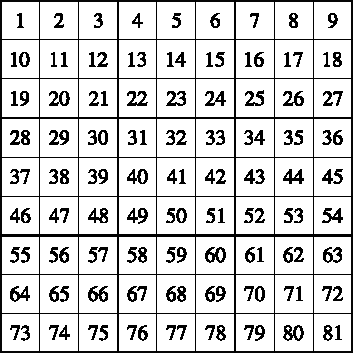
\includegraphics{sudoku-grid}
\caption{Numbering of the grid locations.}
\label{fig:grid}
\end{figure*}

\section{Propositional variables}

In TFL ({\it Truth-Functional Logic}, otherwise known as {\it Propositional Logic}) the smallest item of consideration is a propositional variable, representing a sentence in natural language. We can't refer to locations or cell contents as variables, only as the statements that they're part of.

We therefore need to set up a bunch of propositional variables that represent the assignment of a particular value of a particular cell on the Sudoku grid. We do this by defining a collection of propositional variables of the following form:

$$
\PV{v, p} = \text{``the value $v$ is assigned to cell $p$''}.
$$

Since there are 9 different potential values and 81 cells, we have a total of 729 propositional variables in this form.

Note that although $v$ and $p$ look like variables, they're not variables within TFL. As far as TFL is concerned, these are just 729 different propositional variables that can be either true or false. There is no other relationship between them.

Our aim is to define the relationships by putting together a collection of sentences in TFL that specify how these propositional variables relate to one another.

\section{The rules}

Using these propositional variables we can now start to define the rules of the game.

\subsection{Every cell takes a single value}

We'll start with the rule that states that every cell must contain precisely one value. Starting with cell number 1, we can capture this with the following sentence of TFL:

\begin{align*}
(&\PV{1,1} \lor (\PV{2,1} \lor (\PV{3,1} \lor (\PV{4,1} \lor (\PV{5,1} \lor (\PV{6,1} \lor (\PV{7,1} \lor (\PV{8,1} \lor \PV{9,1})))))))) \\
& \land (\lnot(\PV{1,1} \land \PV{2,1}) \land (\lnot(\PV{1,1} \land \PV{3,1}) \land (\lnot(\PV{1,1} \land \PV{4,1}) \land (\lnot(\PV{1,1} \land \PV{5,1}) \\
& \land (\lnot(\PV{1,1} \land \PV{6,1}) \land (\lnot(\PV{1,1} \land \PV{7,1}) \land (\lnot(\PV{1,1} \land \PV{8,1}) \land (\lnot(\PV{1,1} \land \PV{9,1}) \\
& \land (\lnot(\PV{2,1} \land \PV{3,1}) \land (\lnot(\PV{2,1} \land \PV{4,1}) \land (\lnot(\PV{2,1} \land \PV{5,1}) \land (\lnot(\PV{2,1} \land \PV{6,1}) \\
& \land (\lnot(\PV{2,1} \land \PV{7,1}) \land (\lnot(\PV{2,1} \land \PV{8,1}) \land (\lnot(\PV{2,1} \land \PV{9,1}) \\
& \land (\lnot(\PV{3,1} \land \PV{4,1}) \land (\lnot(\PV{3,1} \land \PV{5,1}) \land (\lnot(\PV{3,1} \land \PV{6,1}) \\
& \land (\lnot(\PV{3,1} \land \PV{7,1}) \land (\lnot(\PV{3,1} \land \PV{8,1}) \land (\lnot(\PV{3,1} \land \PV{9,1}) \\
& \land (\lnot(\PV{4,1} \land \PV{5,1}) \land (\lnot(\PV{4,1} \land \PV{6,1}) \land (\lnot(\PV{4,1} \land \PV{7,1}) \\
& \land (\lnot(\PV{4,1} \land \PV{8,1}) \land (\lnot(\PV{4,1} \land \PV{9,1}) \\
& \land (\lnot(\PV{5,1} \land \PV{6,1}) \land (\lnot(\PV{5,1} \land \PV{7,1}) \land (\lnot(\PV{5,1} \land \PV{8,1}) \land (\lnot(\PV{5,1} \land \PV{9,1}) \\
& \land (\lnot(\PV{6,1} \land \PV{7,1}) \land (\lnot(\PV{6,1} \land \PV{8,1}) \land (\lnot(\PV{6,1} \land \PV{9,1}) \\
& \land (\lnot(\PV{7,1} \land \PV{8,1}) \land (\lnot(\PV{7,1} \land \PV{9,1}) \\
& \land \lnot(\PV{8,1} \land \PV{9,1}))))))))))))))))))))))))))))))))))))
\end{align*}

We can interpret the above sentence as stating two things. The first row states that the first cell is either 1, or 2, or 3, or, \ldots, or 9. In other words the cell must contain a value between 1 and 9 inclusive. The subsequent seven lines are a conjunction of statements of the form $\lnot (\PV{v_1, 1} \land \PV{v_2, 1})$, where $1 \le v_1 < v_2 \le 9$. Each of these states that only one of each pair can be in the cell. With every distinct pair appearing in the list, this ensures that there can be only one value in each cell.

As a sanity check we should have $\combination[9]{2} = \frac{9!}{2! \times (9 - 2)!} = 36$ entries in this second part (we're choosing distinct unordered pairs from 9 possible values), which counting confirms to be the case.

To reduce the amount of ink required, we'll add ellipses to the above and more frequently write it as follows:

\begin{align*}
(\PV{1, 1} & \lor (\PV{2, 1} \lor \cdots \lor \PV{9, 1}) \cdots ) \\
& \land (\lnot(\PV{1, 1} \land \PV{2, 1}) \land (\lnot(\PV{1, 1} \land \PV{3, 1}) \cdots \land \lnot(\PV{8, 1} \land \PV{9, 1})) \cdots )
\end{align*}

The above tells us that cell 1 contains at least one of the values, but no more than one. We'll need one such formula for each cell of the grid, giving 81 in total:
\begin{align*}
(\PV{1, 1} & \lor (\PV{2, 1} \lor \cdots \lor \PV{9, 1}) \cdots ) \\
& \land (\lnot(\PV{1, 1} \land \PV{2, 1}) \land (\lnot(\PV{1, 1} \land \PV{3, 1}) \cdots \land \lnot(\PV{8, 1} \land \PV{9, 1})) \cdots ) , \\
& \qquad \qquad \qquad \qquad \qquad \vdots \\
(\PV{1, n} & \lor (\PV{2, n} \lor \cdots \lor \PV{9, n}) \cdots ) \\
& \land (\lnot(\PV{1, n} \land \PV{2, n}) \land (\lnot(\PV{1, n} \land \PV{3, n}) \cdots \land \lnot(\PV{8, n} \land \PV{9, n})) \cdots ) , \\
& \qquad \qquad \qquad \qquad \qquad \vdots \\
(\PV{1, 81} & \lor (\PV{2, 81} \lor \cdots \lor \PV{9, 81}) \cdots ) \\
& \land (\lnot(\PV{1, 81} \land \PV{2, 81}) \land (\lnot(\PV{1, 81} \land \PV{3, 81}) \cdots \land \lnot(\PV{8, 81} \land \PV{9, 81})) \cdots ) .
\end{align*}

Here we use $n$ as a notational convenience to represent the numbers between 1 and 81 inclusive. If written out in full there would be no variable needed here.

\subsection{Every row has precisely one instance of each number}

Now we get on to the rules of the game as we typically know them. We're going to construct a statement for each row that says the row contains a single instance of each number. To do this we'll need a couple of helper variables. First we set $r$ to be the row number from 1 to 9 inclusive. Second we set $s = (9 \times (r - 1)) + 1$. We can see that $s$ represents the starting location of each row on the left hand side of the board.

Now we can build up a suitable statement for the row $r$:

\begin{align*}
((\PV{1, s} & \lor (\PV{1, s + 1} \lor \cdots \lor \PV{1, s + 8}) \cdots ) \\
& \land (\lnot(\PV{1, s} \land \PV{1, s + 1}) \land (\lnot(\PV{1, s} \land \PV{1, s + 2}) \cdots \land \lnot(\PV{1, s + 7} \land \PV{1, s + 8})) \cdots )) \\
& \qquad \qquad \qquad \qquad \qquad \vdots \\
{} \land ((\PV{n, s} & \lor (\PV{n, s + 1} \lor \cdots \lor \PV{n, s + 8}) \cdots ) \\
& \land (\lnot(\PV{n, s} \land \PV{n, s + 1}) \land (\lnot(\PV{n, s} \land \PV{n, s + 2}) \cdots \land \lnot(\PV{n, s + 7} \land \PV{n, s + 8})) \cdots )) \\
& \qquad \qquad \qquad \qquad \qquad \vdots \\
{} \land ((\PV{9, s} & \lor (\PV{9,s + 1} \lor \cdots \lor \PV{9, s + 8}) \cdots ) \\
& \land (\lnot(\PV{9, s} \land \PV{9, s + 1}) \land (\lnot(\PV{9, s} \land \PV{n, s + 2}) \cdots \land \lnot(\PV{9, s + 7} \land \PV{9, s + 8})) \cdots )) .
\end{align*}

The first says that the column contains precisely one instance of the value 1; the second says it contains precisely one instance of the value 2 and so on. Combined with the fact that every cell takes precisely one value, this fulfils the requirements for the rows.

Once again, $n$ here is used for notational convenience. Once written out in full, the variables $s$ and $n$ would become concrete values.

Since there are nine rows we'll have nine statements like this in total.

\subsection{Every column has precisely one instance of each number}

The case for the columns is similar, we just have to count things a little more carefully because our locations will use a stride of 9. That is, to get from one position in a column to the next, we have to move up in steps of 9 positions.

For this, let us set $c$ to be the number of the column from 1 to 9 inclusive. Now we take $s = c$ to be the starting position of the column at the top of the board.

Our statement can then be the following:

\begin{align*}
((\PV{1, s} & \lor (\PV{1, s + 9} \lor \cdots \lor \PV{1, s + 72}) \cdots ) \\
& \land (\lnot(\PV{1, s} \land \PV{1, s + 9}) \cdots \land \lnot(\PV{1, s + 63} \land \PV{1, s + 72})) \cdots )) \\
& \qquad \qquad \qquad \qquad \qquad \vdots \\
{} \land ((\PV{n, s} & \lor (\PV{n, s + 9} \lor \cdots \lor \PV{n, s + 72}) \cdots ) \\
& \land (\lnot(\PV{n, s} \land \PV{n, s + 9}) \cdots \land \lnot(\PV{n, s + 63} \land \PV{n, s + 72})) \cdots )) \\
& \qquad \qquad \qquad \qquad \qquad \vdots \\
{} \land ((\PV{9, s} & \lor (\PV{9,s + 9} \lor \cdots \lor \PV{9, s + 8}) \cdots ) \\
& \land (\lnot(\PV{9, s} \land \PV{9, s + 9}) \cdots \land \lnot(\PV{9, s + 63} \land \PV{9, s + 72})) \cdots )) .
\end{align*}



As before, since there are nine columns we'll have nine rules like this in total. The values $s$ and $n$ will resolve to concrete numbers for each of these rules.

\subsection{Every block has precisely one instance of each number}

For the equivalent rule for blocks we have to count even more carefully. Let $b$ be the block number from 1 to 9 inclusive. Then we'll set $s$ -- the location of the top left hand corner of a block -- to be the following:
$$
s = (3 \times (((b - 1) \bmod 3)) + \left(27 \times \floor{\frac{b - 1}{3}}\right) + 1 .
$$

Here we use the notation $\floor{x}$ to mean the value $x$ rounded down to the nearest integer. We can now write our block rule for block $b$ as follows:

\begin{align*}
(\PV{1, s} & \lor (\PV{1, s + 1} \lor (\PV{1, s + 2} \\
& \lor (\PV{1, s + 9} \lor (\PV{1, s + 10} \lor (\PV{1, s + 11} \\
& \lor (\PV{1, s + 18} \lor (\PV{1, s + 19} \lor \PV{1, s + 20})))))))) \\
& \land (\lnot(\PV{1, s} \land \PV{1, s + 1}) \cdots \land \lnot(\PV{1, s + 19} \land \PV{1, s + 20})) \cdots )) \\
& \qquad \qquad \qquad \qquad \qquad \vdots \\
(\PV{n, s} & \lor (\PV{n, s + 1} \lor (\PV{n, s + 2} \\
& \lor (\PV{n, s + 9} \lor (\PV{n, s + 10} \lor (\PV{n, s + 11} \\
& \lor (\PV{n, s + 18} \lor (\PV{n, s + 19} \lor \PV{n, s + 20})))))))) \\
& \land (\lnot(\PV{n, s} \land \PV{n, s + 1}) \cdots \land \lnot(\PV{n, s + 19} \land \PV{n, s + 20})) \cdots )) \\
& \qquad \qquad \qquad \qquad \qquad \vdots \\
(\PV{9, s} & \lor (\PV{9, s + 1} \lor (\PV{9, s + 2} \\
& \lor (\PV{9, s + 9} \lor (\PV{9, s + 10} \lor (\PV{9, s + 11} \\
& \lor (\PV{9, s + 18} \lor (\PV{9, s + 19} \lor \PV{9, s + 20})))))))) \\
& \land (\lnot(\PV{9, s} \land \PV{9, s + 1}) \cdots \land \lnot(\PV{9, s + 19} \land \PV{9, s + 20})) \cdots )) \\
\end{align*}

There are nine blocks, so once again we have nine of these rules. All of the instances of $s$ and $n$ will resolve to concrete values when written out in full.

\subsection{The initial board position}

This gives us the rules of the game: 108 rules in total. All we need now is to bring in the actual game board. Let's suppose, for the sake of example, that the initial state of the board is as shown in Figure \ref{fig:initial}.

\begin{figure*}[h!]
\centering
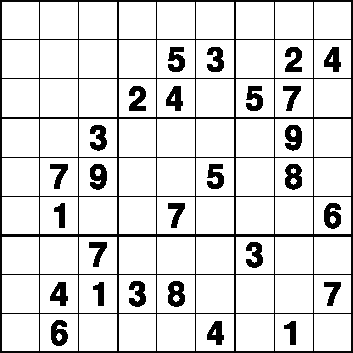
\includegraphics{sudoku-01}
\caption{An example game board.}
\label{fig:initial}
\end{figure*}

This has 27 of the 81 cells with numbers already filled in. We can use our propositional variables to describe this state as well. Comparing figures \ref{fig:grid} and \ref{fig:initial} we can see that cell 14 contains the value 5, cell 15 contains the value 3, cell 17 contains the value 2 and so on. We can write these as follows:

\begin{align*}
\PV{5, 14} & \land (\PV{3, 15} \land (\PV{2, 17} \land (\PV{4, 18} \\
& \land (\PV{2, 22} \land (\PV{4, 23} \land (\PV{5, 25} \land (\PV{7, 26} \\
& \land (\PV{3, 30} \land (\PV{9, 35} \\
& \land (\PV{7, 38} \land (\PV{9, 39} \land (\PV{5, 42} \land (\PV{8, 44} \\
& \land (\PV{1, 47} \land (\PV{7, 50} \land (\PV{6, 54} \\
& \land (\PV{7, 57} \land (\PV{3, 61} \\
& \land (\PV{4, 65} \land (\PV{1, 66} \land (\PV{3, 67} \land (\PV{8, 68} \land (\PV{7, 72} \\
& \land (\PV{6, 74} \land (\PV{4, 78} \land (\PV{1, 80} )))))))))))))))))))))))))).
\end{align*}

\subsection{Serialising}

The numbers we use to refer to the propositional variables can be simplified by setting up the following rule:
$$
\QV{n} = \PV{((n - 1) \bmod 9) + 1, \floor{\frac{n - 1}{9}} + 1}
$$

In other words, if $v$ is the value and $p$ is the position then $\PV{v, p} = \QV{n}$ where $n = v + (9 \times (p - 1))$.

We could convert all of the above statements to use this notation, but skip doing so because it's rather tedious and not very helpful for actually understanding what's going on.

\subsection{Solving the puzzle with truth tables}

If we combine all of these 109 rules together, we could write out the truth table for them. With 729 propositional variables there would be
$$
2^{729} = 2.824 \times 10^{219}
$$
rows (approximately 3 duoseptuagintillion), which is rather a large truth table.

Nevertheless, for a well-formed puzzle, only one of the rows of the truth table will contain all {\it true} values on the right hand side of the table. This would represent the correct solution to the puzzle.

Of course, we can also simplify our truth table considerably, because we know all of the 27 initial position statements have to be {\it true} and all of the propositional values for the same positions but different numbers have to be false. This fixes 243 of our propositional values, leaving just 486 that we have to consider. Our truth table is now just
$$
2^{486} = 1.9979 \times 10^{146}
$$
rows (a mere 200 septenquadragintillion).

\subsection{Solving the puzzle with deduction}

Rather than go through all of the lines of the truth table, an alternative approach is to apply rules of deduction in an attempt to simplify the formula. For example, consider the following rules:

\begin{align*}
\meta{P} \rightarrow \meta{Q}, \meta{P} & \vdash \meta{Q} \\
\meta{P} \land \meta{Q}, \meta{P} & \vdash \meta{Q} \\
\meta{P} \land \meta{Q}, \meta{Q} & \vdash \meta{P} \\
\meta{P} \lor \meta{Q}, \lnot \meta{P} & \vdash \meta{Q} \\
\meta{P} \lor \meta{Q}, \lnot \meta{Q} & \vdash \meta{P}
\end{align*}

Since these are all valid arguments, whenever we find a pattern that looks like the left hand side, we can replace it with the sentence on the right hand side without affecting the truth of the statement.

Using a deduction engine to repeatedly apply these and other rules, the original sentence containing 64205 connectives was reduced down to a sentence containing 3268 connectives.

In the process, the following propositions were found to be {\it true} by the deduction engine:

\begin{align*}
& \PV{5,2},_{\hphantom{1}} \PV{7,6},_{\hphantom{1}} \PV{6,8},_{\hphantom{1}} \PV{3,9},_{\hphantom{,}} \PV{7,10}, \\
& \PV{5,14}, \PV{3,15}, \PV{2,17}, \PV{4,18}, \PV{3,20}, \\
& \PV{2,22}, \PV{4,23}, \PV{5,25}, \PV{7,26}, \PV{3,30}, \\
& \PV{7,34}, \PV{9,35}, \PV{5,36}, \PV{7,38}, \PV{9,39}, \\
& \PV{3,41}, \PV{5,42}, \PV{8,44}, \PV{5,46}, \PV{1,47}, \\
& \PV{7,50}, \PV{3,53}, \PV{6,54}, \PV{7,57}, \PV{5,58}, \\
& \PV{3,61}, \PV{4,62}, \PV{4,65}, \PV{1,66}, \PV{3,67}, \\
& \PV{8,68}, \PV{6,70}, \PV{5,71}, \PV{7,72}, \PV{3,73}, \\
& \PV{6,74}, \PV{5,75}, \PV{7,76}, \PV{4,78}, \PV{1,80}.
\end{align*}

Each of these represents a statement about the Sudoku board, so we can apply these to the grid to make progress with the puzzle. The resulting Sudoku board can be seen in Figure \ref{fig:partial}.

\begin{figure*}[h!]
\centering
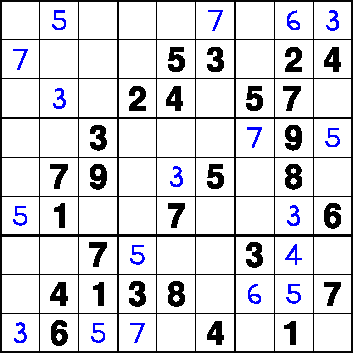
\includegraphics{sudoku-02}
\caption{Partially solved Sudoku puzzle.}
\label{fig:partial}
\end{figure*}

In theory it should be possible to manipulate the sentence and apply further deduction rules to solve the puzzle in full, but I've not been able to find deduction rules to take the puzzle beyond these obvious first steps.

The remaining 3268-connective sentence containing only the propositions that couldn't be determined is shown below.

Having determined the values of 45 out of the 81 cells, our truth table now needs only $2^{324} = 3.418 \times 10^{97}$ rows (34 untrigintillion).

\begin{align*}
& (((((((((((((((((((((((((((((((((((((((((((((((((((((((((((((((((((((((((((\PV{1,1} \\
& \lor \PV{2,1}) \lor \PV{4,1}) \lor \PV{8,1}) \lor \PV{9,1}) \land \lnot(\PV{1,1} \land \PV{2,1})) \land \lnot(\PV{1,1} \land \PV{4,1})) \land \lnot(\PV{1,1} \\
& \land \PV{8,1})) \land \lnot(\PV{1,1} \land \PV{9,1})) \land \lnot(\PV{2,1} \land \PV{4,1})) \land \lnot(\PV{2,1} \land \PV{8,1})) \land \lnot(\PV{2,1} \\
& \land \PV{9,1})) \land \lnot(\PV{4,1} \land \PV{8,1})) \land \lnot(\PV{4,1} \land \PV{9,1})) \land \lnot(\PV{8,1} \land \PV{9,1})) \land (((((\PV{2,3} \\
& \lor \PV{4,3}) \lor \PV{8,3}) \land \lnot(\PV{2,3} \land \PV{4,3})) \land \lnot(\PV{2,3} \land \PV{8,3})) \land \lnot(\PV{4,3} \land \PV{8,3}))) \\
& \land (((((\PV{1,4} \lor \PV{8,4}) \lor \PV{9,4}) \land \lnot(\PV{1,4} \land \PV{8,4})) \land \lnot(\PV{1,4} \land \PV{9,4})) \\
& \land \lnot(\PV{8,4} \land \PV{9,4}))) \land ((\PV{1,5} \lor \PV{9,5}) \land \lnot(\PV{1,5} \land \PV{9,5}))) \land (((((\PV{1,7} \\
& \lor \PV{8,7}) \lor \PV{9,7}) \land \lnot(\PV{1,7} \land \PV{8,7})) \land \lnot(\PV{1,7} \land \PV{9,7})) \land \lnot(\PV{8,7} \land \PV{9,7}))) \\
& \land ((\PV{8,11} \lor \PV{9,11}) \land \lnot(\PV{8,11} \land \PV{9,11}))) \land ((\PV{6,12} \lor \PV{8,12}) \land \lnot(\PV{6,12} \\
& \land \PV{8,12}))) \land (((((((((\PV{1,13} \lor \PV{6,13}) \lor \PV{8,13}) \lor \PV{9,13}) \land \lnot(\PV{1,13} \\
& \land \PV{6,13})) \land \lnot(\PV{1,13} \land \PV{8,13})) \land \lnot(\PV{1,13} \land \PV{9,13})) \land \lnot(\PV{6,13} \land \PV{8,13})) \\
& \land \lnot(\PV{6,13} \land \PV{9,13})) \land \lnot(\PV{8,13} \land \PV{9,13}))) \land (((((\PV{1,16} \lor \PV{8,16}) \\
& \lor \PV{9,16}) \land \lnot(\PV{1,16} \land \PV{8,16})) \land \lnot(\PV{1,16} \land \PV{9,16})) \land \lnot(\PV{8,16} \land \PV{9,16}))) \\
& \land (((((((((\PV{1,19} \lor \PV{6,19}) \lor \PV{8,19}) \lor \PV{9,19}) \land \lnot(\PV{1,19} \land \PV{6,19})) \\
& \land \lnot(\PV{1,19} \land \PV{8,19})) \land \lnot(\PV{1,19} \land \PV{9,19})) \land \lnot(\PV{6,19} \land \PV{8,19})) \land \lnot(\PV{6,19} \\
& \land \PV{9,19})) \land \lnot(\PV{8,19} \land \PV{9,19}))) \land ((\PV{6,21} \lor \PV{8,21}) \land \lnot(\PV{6,21} \land \PV{8,21}))) \\
& \land (((((((((\PV{1,24} \lor \PV{6,24}) \lor \PV{8,24}) \lor \PV{9,24}) \land \lnot(\PV{1,24} \land \PV{6,24})) \\
& \land \lnot(\PV{1,24} \land \PV{8,24})) \land \lnot(\PV{1,24} \land \PV{9,24})) \land \lnot(\PV{6,24} \land \PV{8,24})) \land \lnot(\PV{6,24} \\
& \land \PV{9,24})) \land \lnot(\PV{8,24} \land \PV{9,24}))) \land (((((\PV{1,27} \lor \PV{8,27}) \lor \PV{9,27}) \land \lnot(\PV{1,27} \\
& \land \PV{8,27})) \land \lnot(\PV{1,27} \land \PV{9,27})) \land \lnot(\PV{8,27} \land \PV{9,27}))) \land (((((((((\PV{2,28} \\
& \lor \PV{4,28}) \lor \PV{6,28}) \lor \PV{8,28}) \land \lnot(\PV{2,28} \land \PV{4,28})) \land \lnot(\PV{2,28} \land \PV{6,28})) \land \lnot(\PV{2,28} \\
& \land \PV{8,28})) \land \lnot(\PV{4,28} \land \PV{6,28})) \land \lnot(\PV{4,28} \land \PV{8,28})) \land \lnot(\PV{6,28} \land \PV{8,28}))) \\
& \land ((\PV{2,29} \lor \PV{8,29}) \land \lnot(\PV{2,29} \land \PV{8,29}))) \land (((((((((\PV{1,31} \\
& \lor \PV{4,31}) \lor \PV{6,31}) \lor \PV{8,31}) \land \lnot(\PV{1,31} \land \PV{4,31})) \land \lnot(\PV{1,31} \land \PV{6,31})) \land \lnot(\PV{1,31} \\
& \land \PV{8,31})) \land \lnot(\PV{4,31} \land \PV{6,31})) \land \lnot(\PV{4,31} \land \PV{8,31})) \land \lnot(\PV{6,31} \land \PV{8,31}))) \\
& \land (((((\PV{1,32} \lor \PV{2,32}) \lor \PV{6,32}) \land \lnot(\PV{1,32} \land \PV{2,32})) \land \lnot(\PV{1,32} \land \PV{6,32})) \\
& \land \lnot(\PV{2,32} \land \PV{6,32}))) \land (((((((((\PV{1,33} \lor \PV{2,33}) \lor \PV{6,33}) \\
& \lor \PV{8,33}) \land \lnot(\PV{1,33} \land \PV{2,33})) \land \lnot(\PV{1,33} \land \PV{6,33})) \land \lnot(\PV{1,33} \land \PV{8,33})) \\
& \land \lnot(\PV{2,33} \land \PV{6,33})) \land \lnot(\PV{2,33} \land \PV{8,33})) \land \lnot(\PV{6,33} \land \PV{8,33}))) \land (((((\PV{2,37} \\
& \lor \PV{4,37}) \lor \PV{6,37}) \land \lnot(\PV{2,37} \land \PV{4,37})) \land \lnot(\PV{2,37} \land \PV{6,37})) \land \lnot(\PV{4,37} \land \PV{6,37}))) \\
& \land (((((\PV{1,40} \lor \PV{4,40}) \lor \PV{6,40}) \land \lnot(\PV{1,40} \land \PV{4,40})) \land \lnot(\PV{1,40} \land \PV{6,40})) \\
& \land \lnot(\PV{4,40} \land \PV{6,40}))) \land (((((\PV{1,43} \lor \PV{2,43}) \lor \PV{4,43}) \land \lnot(\PV{1,43} \\
& \land \PV{2,43})) \land \lnot(\PV{1,43} \land \PV{4,43})) \land \lnot(\PV{2,43} \land \PV{4,43}))) \land ((\PV{1,45} \lor \PV{2,45}) \\
& \land \lnot(\PV{1,45} \land \PV{2,45}))) \land (((((\PV{2,48} \lor \PV{4,48}) \lor \PV{8,48}) \land \lnot(\PV{2,48} \\
& \land \PV{4,48})) \land \lnot(\PV{2,48} \land \PV{8,48})) \land \lnot(\PV{4,48} \land \PV{8,48}))) \land (((((\PV{4,49} \\
& \lor \PV{8,49}) \lor \PV{9,49}) \land \lnot(\PV{4,49} \land \PV{8,49})) \land \lnot(\PV{4,49} \land \PV{9,49})) \land \lnot(\PV{8,49} \land \PV{9,49}))) \\
& \land (((((\PV{2,51} \lor \PV{8,51}) \lor \PV{9,51}) \land \lnot(\PV{2,51} \land \PV{8,51})) \land \lnot(\PV{2,51} \land \PV{9,51})) \\
& \land \lnot(\PV{8,51} \land \PV{9,51}))) \land ((\PV{2,52} \lor \PV{4,52}) \land \lnot(\PV{2,52} \land \PV{4,52}))) \land (((((\PV{2,55} \\
& \lor \PV{8,55}) \lor \PV{9,55}) \land \lnot(\PV{2,55} \land \PV{8,55})) \land \lnot(\PV{2,55} \land \PV{9,55})) \land \lnot(\PV{8,55} \land \PV{9,55}))) \\
& \land (((((\PV{2,56} \lor \PV{8,56}) \lor \PV{9,56}) \land \lnot(\PV{2,56} \land \PV{8,56})) \land \lnot(\PV{2,56} \land \PV{9,56})) \\
& \land \lnot(\PV{8,56} \land \PV{9,56}))) \land (((((((((\PV{1,59} \lor \PV{2,59}) \lor \PV{6,59}) \\
& \lor \PV{9,59}) \land \lnot(\PV{1,59} \land \PV{2,59})) \land \lnot(\PV{1,59} \land \PV{6,59})) \land \lnot(\PV{1,59} \land \PV{9,59})) \\
& \land \lnot(\PV{2,59} \land \PV{6,59})) \land \lnot(\PV{2,59} \land \PV{9,59})) \land \lnot(\PV{6,59} \land \PV{9,59}))) \land (((((((((\PV{1,60} \\
& \lor \PV{2,60}) \lor \PV{6,60}) \lor \PV{9,60}) \land \lnot(\PV{1,60} \land \PV{2,60})) \land \lnot(\PV{1,60} \land \PV{6,60})) \land \lnot(\PV{1,60} \\
& \land \PV{9,60})) \land \lnot(\PV{2,60} \land \PV{6,60})) \land \lnot(\PV{2,60} \land \PV{9,60})) \land \lnot(\PV{6,60} \land \PV{9,60}))) \\
& \land (((((\PV{2,63} \lor \PV{8,63}) \lor \PV{9,63}) \land \lnot(\PV{2,63} \land \PV{8,63})) \land \lnot(\PV{2,63} \land \PV{9,63})) \\
& \land \lnot(\PV{8,63} \land \PV{9,63}))) \land ((\PV{2,64} \lor \PV{9,64}) \land \lnot(\PV{2,64} \land \PV{9,64}))) \land ((\PV{2,69} \\
& \lor \PV{9,69}) \land \lnot(\PV{2,69} \land \PV{9,69}))) \land ((\PV{2,77} \lor \PV{9,77}) \land \lnot(\PV{2,77} \land \PV{9,77}))) \\
& \land (((((\PV{2,79} \lor \PV{8,79}) \lor \PV{9,79}) \land \lnot(\PV{2,79} \land \PV{8,79})) \land \lnot(\PV{2,79} \land \PV{9,79})) \\
& \land \lnot(\PV{8,79} \land \PV{9,79}))) \land (((((\PV{2,81} \lor \PV{8,81}) \lor \PV{9,81}) \land \lnot(\PV{2,81} \\
& \land \PV{8,81})) \land \lnot(\PV{2,81} \land \PV{9,81})) \land \lnot(\PV{8,81} \land \PV{9,81}))) \land (((((((((((((\PV{1,7} \\
& \lor \PV{1,5}) \lor \PV{1,4}) \lor \PV{1,1}) \land \lnot(\PV{1,7} \land \PV{1,5})) \land \lnot(\PV{1,7} \land \PV{1,4})) \land \lnot(\PV{1,7} \\
& \land \PV{1,1})) \land \lnot(\PV{1,5} \land \PV{1,4})) \land \lnot(\PV{1,5} \land \PV{1,1})) \land \lnot(\PV{1,4} \land \PV{1,1})) \land ((\PV{2,3} \\
& \lor \PV{2,1}) \land \lnot(\PV{2,3} \land \PV{2,1}))) \land ((\PV{4,3} \lor \PV{4,1}) \land \lnot(\PV{4,3} \land \PV{4,1}))) \land (((((((((\PV{8,7} \\
& \lor \PV{8,4}) \lor \PV{8,3}) \lor \PV{8,1}) \land \lnot(\PV{8,7} \land \PV{8,4})) \land \lnot(\PV{8,7} \land \PV{8,3})) \land \lnot(\PV{8,7} \\
& \land \PV{8,1})) \land \lnot(\PV{8,4} \land \PV{8,3})) \land \lnot(\PV{8,4} \land \PV{8,1})) \land \lnot(\PV{8,3} \land \PV{8,1}))) \\
& \land (((((((((\PV{9,7} \lor \PV{9,5}) \lor \PV{9,4}) \lor \PV{9,1}) \land \lnot(\PV{9,7} \land \PV{9,5})) \\
& \land \lnot(\PV{9,7} \land \PV{9,4})) \land \lnot(\PV{9,7} \land \PV{9,1})) \land \lnot(\PV{9,5} \land \PV{9,4})) \land \lnot(\PV{9,5} \\
& \land \PV{9,1})) \land \lnot(\PV{9,4} \land \PV{9,1})))) \land (((((\PV{1,16} \lor \PV{1,13}) \land \lnot(\PV{1,16} \\
& \land \PV{1,13})) \land ((\PV{6,13} \lor \PV{6,12}) \land \lnot(\PV{6,13} \land \PV{6,12}))) \land (((((((((\PV{8,16} \\
& \lor \PV{8,13}) \lor \PV{8,12}) \lor \PV{8,11}) \land \lnot(\PV{8,16} \land \PV{8,13})) \land \lnot(\PV{8,16} \land \PV{8,12})) \land \lnot(\PV{8,16} \\
& \land \PV{8,11})) \land \lnot(\PV{8,13} \land \PV{8,12})) \land \lnot(\PV{8,13} \land \PV{8,11})) \land \lnot(\PV{8,12} \land \PV{8,11}))) \\
& \land (((((\PV{9,16} \lor \PV{9,13}) \lor \PV{9,11}) \land \lnot(\PV{9,16} \land \PV{9,13})) \land \lnot(\PV{9,16} \land \PV{9,11})) \\
& \land \lnot(\PV{9,13} \land \PV{9,11})))) \land ((((((((\PV{1,27} \lor \PV{1,24}) \lor \PV{1,19}) \\
& \land \lnot(\PV{1,27} \land \PV{1,24})) \land \lnot(\PV{1,27} \land \PV{1,19})) \land \lnot(\PV{1,24} \land \PV{1,19})) \land (((((\PV{6,24} \\
& \lor \PV{6,21}) \lor \PV{6,19}) \land \lnot(\PV{6,24} \land \PV{6,21})) \land \lnot(\PV{6,24} \land \PV{6,19})) \land \lnot(\PV{6,21} \land \PV{6,19}))) \\
& \land (((((((((\PV{8,27} \lor \PV{8,24}) \lor \PV{8,21}) \lor \PV{8,19}) \land \lnot(\PV{8,27} \land \PV{8,24})) \\
& \land \lnot(\PV{8,27} \land \PV{8,21})) \land \lnot(\PV{8,27} \land \PV{8,19})) \land \lnot(\PV{8,24} \land \PV{8,21})) \land \lnot(\PV{8,24} \\
& \land \PV{8,19})) \land \lnot(\PV{8,21} \land \PV{8,19}))) \land (((((\PV{9,27} \lor \PV{9,24}) \lor \PV{9,19}) \land \lnot(\PV{9,27} \\
& \land \PV{9,24})) \land \lnot(\PV{9,27} \land \PV{9,19})) \land \lnot(\PV{9,24} \land \PV{9,19})))) \land (((((((((\PV{1,33} \\
& \lor \PV{1,32}) \lor \PV{1,31}) \land \lnot(\PV{1,33} \land \PV{1,32})) \land \lnot(\PV{1,33} \land \PV{1,31})) \land \lnot(\PV{1,32} \land \PV{1,31})) \\
& \land (((((((((\PV{2,33} \lor \PV{2,32}) \lor \PV{2,29}) \lor \PV{2,28}) \land \lnot(\PV{2,33} \land \PV{2,32})) \\
& \land \lnot(\PV{2,33} \land \PV{2,29})) \land \lnot(\PV{2,33} \land \PV{2,28})) \land \lnot(\PV{2,32} \land \PV{2,29})) \land \lnot(\PV{2,32} \\
& \land \PV{2,28})) \land \lnot(\PV{2,29} \land \PV{2,28}))) \land ((\PV{4,31} \lor \PV{4,28}) \land \lnot(\PV{4,31} \land \PV{4,28}))) \\
& \land (((((((((\PV{6,33} \lor \PV{6,32}) \lor \PV{6,31}) \lor \PV{6,28}) \land \lnot(\PV{6,33} \land \PV{6,32})) \\
& \land \lnot(\PV{6,33} \land \PV{6,31})) \land \lnot(\PV{6,33} \land \PV{6,28})) \land \lnot(\PV{6,32} \land \PV{6,31})) \land \lnot(\PV{6,32} \\
& \land \PV{6,28})) \land \lnot(\PV{6,31} \land \PV{6,28}))) \land (((((((((\PV{8,33} \lor \PV{8,31}) \\
& \lor \PV{8,29}) \lor \PV{8,28}) \land \lnot(\PV{8,33} \land \PV{8,31})) \land \lnot(\PV{8,33} \land \PV{8,29})) \land \lnot(\PV{8,33} \land \PV{8,28})) \\
& \land \lnot(\PV{8,31} \land \PV{8,29})) \land \lnot(\PV{8,31} \land \PV{8,28})) \land \lnot(\PV{8,29} \land \PV{8,28})))) \land ((((((((\PV{1,45} \\
& \lor \PV{1,43}) \lor \PV{1,40}) \land \lnot(\PV{1,45} \land \PV{1,43})) \land \lnot(\PV{1,45} \land \PV{1,40})) \land \lnot(\PV{1,43} \land \PV{1,40})) \\
& \land (((((\PV{2,45} \lor \PV{2,43}) \lor \PV{2,37}) \land \lnot(\PV{2,45} \land \PV{2,43})) \land \lnot(\PV{2,45} \land \PV{2,37})) \\
& \land \lnot(\PV{2,43} \land \PV{2,37}))) \land (((((\PV{4,43} \lor \PV{4,40}) \lor \PV{4,37}) \land \lnot(\PV{4,43} \\
& \land \PV{4,40})) \land \lnot(\PV{4,43} \land \PV{4,37})) \land \lnot(\PV{4,40} \land \PV{4,37}))) \land ((\PV{6,40} \lor \PV{6,37}) \\
& \land \lnot(\PV{6,40} \land \PV{6,37})))) \land ((((((((\PV{2,52} \lor \PV{2,51}) \lor \PV{2,48}) \\
& \land \lnot(\PV{2,52} \land \PV{2,51})) \land \lnot(\PV{2,52} \land \PV{2,48})) \land \lnot(\PV{2,51} \land \PV{2,48})) \land (((((\PV{4,52} \\
& \lor \PV{4,49}) \lor \PV{4,48}) \land \lnot(\PV{4,52} \land \PV{4,49})) \land \lnot(\PV{4,52} \land \PV{4,48})) \land \lnot(\PV{4,49} \land \PV{4,48}))) \\
& \land (((((\PV{8,51} \lor \PV{8,49}) \lor \PV{8,48}) \land \lnot(\PV{8,51} \land \PV{8,49})) \land \lnot(\PV{8,51} \land \PV{8,48})) \\
& \land \lnot(\PV{8,49} \land \PV{8,48}))) \land ((\PV{9,51} \lor \PV{9,49}) \land \lnot(\PV{9,51} \land \PV{9,49})))) \land ((((((\PV{1,60} \\
& \lor \PV{1,59}) \land \lnot(\PV{1,60} \land \PV{1,59})) \land ((((((((((((((\PV{2,63} \\
& \lor \PV{2,60}) \lor \PV{2,59}) \lor \PV{2,56}) \lor \PV{2,55}) \land \lnot(\PV{2,63} \land \PV{2,60})) \land \lnot(\PV{2,63} \land \PV{2,59})) \\
& \land \lnot(\PV{2,63} \land \PV{2,56})) \land \lnot(\PV{2,63} \land \PV{2,55})) \land \lnot(\PV{2,60} \land \PV{2,59})) \land \lnot(\PV{2,60} \\
& \land \PV{2,56})) \land \lnot(\PV{2,60} \land \PV{2,55})) \land \lnot(\PV{2,59} \land \PV{2,56})) \land \lnot(\PV{2,59} \land \PV{2,55})) \\
& \land \lnot(\PV{2,56} \land \PV{2,55}))) \land ((\PV{6,60} \lor \PV{6,59}) \land \lnot(\PV{6,60} \land \PV{6,59}))) \land (((((\PV{8,63} \\
& \lor \PV{8,56}) \lor \PV{8,55}) \land \lnot(\PV{8,63} \land \PV{8,56})) \land \lnot(\PV{8,63} \land \PV{8,55})) \land \lnot(\PV{8,56} \land \PV{8,55}))) \\
& \land ((((((((((((((\PV{9,63} \lor \PV{9,60}) \lor \PV{9,59}) \lor \PV{9,56}) \\
& \lor \PV{9,55}) \land \lnot(\PV{9,63} \land \PV{9,60})) \land \lnot(\PV{9,63} \land \PV{9,59})) \land \lnot(\PV{9,63} \land \PV{9,56})) \\
& \land \lnot(\PV{9,63} \land \PV{9,55})) \land \lnot(\PV{9,60} \land \PV{9,59})) \land \lnot(\PV{9,60} \land \PV{9,56})) \land \lnot(\PV{9,60} \\
& \land \PV{9,55})) \land \lnot(\PV{9,59} \land \PV{9,56})) \land \lnot(\PV{9,59} \land \PV{9,55})) \land \lnot(\PV{9,56} \land \PV{9,55})))) \\
& \land (((\PV{2,69} \lor \PV{2,64}) \land \lnot(\PV{2,69} \land \PV{2,64})) \land ((\PV{9,69} \lor \PV{9,64}) \land \lnot(\PV{9,69} \\
& \land \PV{9,64})))) \land (((((((\PV{2,81} \lor \PV{2,79}) \lor \PV{2,77}) \land \lnot(\PV{2,81} \land \PV{2,79})) \\
& \land \lnot(\PV{2,81} \land \PV{2,77})) \land \lnot(\PV{2,79} \land \PV{2,77})) \land ((\PV{8,81} \lor \PV{8,79}) \land \lnot(\PV{8,81} \\
& \land \PV{8,79}))) \land (((((\PV{9,81} \lor \PV{9,79}) \lor \PV{9,77}) \land \lnot(\PV{9,81} \land \PV{9,79})) \land \lnot(\PV{9,81} \\
& \land \PV{9,77})) \land \lnot(\PV{9,79} \land \PV{9,77})))) \land (((((((\PV{1,19} \lor \PV{1,1}) \land \lnot(\PV{1,19} \\
& \land \PV{1,1})) \land ((((((((((((((\PV{2,64} \lor \PV{2,55}) \lor \PV{2,37}) \\
& \lor \PV{2,28}) \lor \PV{2,1}) \land \lnot(\PV{2,64} \land \PV{2,55})) \land \lnot(\PV{2,64} \land \PV{2,37})) \land \lnot(\PV{2,64} \land \PV{2,28})) \\
& \land \lnot(\PV{2,64} \land \PV{2,1})) \land \lnot(\PV{2,55} \land \PV{2,37})) \land \lnot(\PV{2,55} \land \PV{2,28})) \land \lnot(\PV{2,55} \\
& \land \PV{2,1})) \land \lnot(\PV{2,37} \land \PV{2,28})) \land \lnot(\PV{2,37} \land \PV{2,1})) \land \lnot(\PV{2,28} \land \PV{2,1}))) \\
& \land (((((\PV{4,37} \lor \PV{4,28}) \lor \PV{4,1}) \land \lnot(\PV{4,37} \land \PV{4,28})) \land \lnot(\PV{4,37} \land \PV{4,1})) \\
& \land \lnot(\PV{4,28} \land \PV{4,1}))) \land (((((\PV{6,37} \lor \PV{6,28}) \lor \PV{6,19}) \land \lnot(\PV{6,37} \\
& \land \PV{6,28})) \land \lnot(\PV{6,37} \land \PV{6,19})) \land \lnot(\PV{6,28} \land \PV{6,19}))) \land (((((((((\PV{8,55} \\
& \lor \PV{8,28}) \lor \PV{8,19}) \lor \PV{8,1}) \land \lnot(\PV{8,55} \land \PV{8,28})) \land \lnot(\PV{8,55} \land \PV{8,19})) \land \lnot(\PV{8,55} \\
& \land \PV{8,1})) \land \lnot(\PV{8,28} \land \PV{8,19})) \land \lnot(\PV{8,28} \land \PV{8,1})) \land \lnot(\PV{8,19} \land \PV{8,1}))) \\
& \land (((((((((\PV{9,64} \lor \PV{9,55}) \lor \PV{9,19}) \lor \PV{9,1}) \land \lnot(\PV{9,64} \land \PV{9,55})) \\
& \land \lnot(\PV{9,64} \land \PV{9,19})) \land \lnot(\PV{9,64} \land \PV{9,1})) \land \lnot(\PV{9,55} \land \PV{9,19})) \land \lnot(\PV{9,55} \\
& \land \PV{9,1})) \land \lnot(\PV{9,19} \land \PV{9,1})))) \land ((((\PV{2,56} \lor \PV{2,29}) \land \lnot(\PV{2,56} \\
& \land \PV{2,29})) \land (((((\PV{8,56} \lor \PV{8,29}) \lor \PV{8,11}) \land \lnot(\PV{8,56} \land \PV{8,29})) \land \lnot(\PV{8,56} \\
& \land \PV{8,11})) \land \lnot(\PV{8,29} \land \PV{8,11}))) \land ((\PV{9,56} \lor \PV{9,11}) \land \lnot(\PV{9,56} \land \PV{9,11})))) \\
& \land (((((\PV{2,48} \lor \PV{2,3}) \land \lnot(\PV{2,48} \land \PV{2,3})) \land ((\PV{4,48} \lor \PV{4,3}) \land \lnot(\PV{4,48} \\
& \land \PV{4,3}))) \land ((\PV{6,21} \lor \PV{6,12}) \land \lnot(\PV{6,21} \land \PV{6,12}))) \land (((((((((\PV{8,48} \\
& \lor \PV{8,21}) \lor \PV{8,12}) \lor \PV{8,3}) \land \lnot(\PV{8,48} \land \PV{8,21})) \land \lnot(\PV{8,48} \land \PV{8,12})) \land \lnot(\PV{8,48} \\
& \land \PV{8,3})) \land \lnot(\PV{8,21} \land \PV{8,12})) \land \lnot(\PV{8,21} \land \PV{8,3})) \land \lnot(\PV{8,12} \land \PV{8,3})))) \\
& \land (((((((((((((\PV{1,40} \lor \PV{1,31}) \lor \PV{1,13}) \lor \PV{1,4}) \land \lnot(\PV{1,40} \\
& \land \PV{1,31})) \land \lnot(\PV{1,40} \land \PV{1,13})) \land \lnot(\PV{1,40} \land \PV{1,4})) \land \lnot(\PV{1,31} \land \PV{1,13})) \\
& \land \lnot(\PV{1,31} \land \PV{1,4})) \land \lnot(\PV{1,13} \land \PV{1,4})) \land (((((\PV{4,49} \lor \PV{4,40}) \\
& \lor \PV{4,31}) \land \lnot(\PV{4,49} \land \PV{4,40})) \land \lnot(\PV{4,49} \land \PV{4,31})) \land \lnot(\PV{4,40} \land \PV{4,31}))) \\
& \land (((((\PV{6,40} \lor \PV{6,31}) \lor \PV{6,13}) \land \lnot(\PV{6,40} \land \PV{6,31})) \land \lnot(\PV{6,40} \land \PV{6,13})) \\
& \land \lnot(\PV{6,31} \land \PV{6,13}))) \land (((((((((\PV{8,49} \lor \PV{8,31}) \lor \PV{8,13}) \\
& \lor \PV{8,4}) \land \lnot(\PV{8,49} \land \PV{8,31})) \land \lnot(\PV{8,49} \land \PV{8,13})) \land \lnot(\PV{8,49} \land \PV{8,4})) \land \lnot(\PV{8,31} \\
& \land \PV{8,13})) \land \lnot(\PV{8,31} \land \PV{8,4})) \land \lnot(\PV{8,13} \land \PV{8,4}))) \land (((((\PV{9,49} \\
& \lor \PV{9,13}) \lor \PV{9,4}) \land \lnot(\PV{9,49} \land \PV{9,13})) \land \lnot(\PV{9,49} \land \PV{9,4})) \land \lnot(\PV{9,13} \land \PV{9,4})))) \\
& \land ((((((((\PV{1,59} \lor \PV{1,32}) \lor \PV{1,5}) \land \lnot(\PV{1,59} \land \PV{1,32})) \land \lnot(\PV{1,59} \\
& \land \PV{1,5})) \land \lnot(\PV{1,32} \land \PV{1,5})) \land (((((\PV{2,77} \lor \PV{2,59}) \lor \PV{2,32}) \land \lnot(\PV{2,77} \\
& \land \PV{2,59})) \land \lnot(\PV{2,77} \land \PV{2,32})) \land \lnot(\PV{2,59} \land \PV{2,32}))) \land ((\PV{6,59} \lor \PV{6,32}) \\
& \land \lnot(\PV{6,59} \land \PV{6,32}))) \land (((((\PV{9,77} \lor \PV{9,59}) \lor \PV{9,5}) \land \lnot(\PV{9,77} \\
& \land \PV{9,59})) \land \lnot(\PV{9,77} \land \PV{9,5})) \land \lnot(\PV{9,59} \land \PV{9,5})))) \land (((((((((\PV{1,60} \\
& \lor \PV{1,33}) \lor \PV{1,24}) \land \lnot(\PV{1,60} \land \PV{1,33})) \land \lnot(\PV{1,60} \land \PV{1,24})) \land \lnot(\PV{1,33} \land \PV{1,24})) \\
& \land (((((((((\PV{2,69} \lor \PV{2,60}) \lor \PV{2,51}) \lor \PV{2,33}) \land \lnot(\PV{2,69} \land \PV{2,60})) \\
& \land \lnot(\PV{2,69} \land \PV{2,51})) \land \lnot(\PV{2,69} \land \PV{2,33})) \land \lnot(\PV{2,60} \land \PV{2,51})) \land \lnot(\PV{2,60} \\
& \land \PV{2,33})) \land \lnot(\PV{2,51} \land \PV{2,33}))) \land (((((\PV{6,60} \lor \PV{6,33}) \lor \PV{6,24}) \land \lnot(\PV{6,60} \\
& \land \PV{6,33})) \land \lnot(\PV{6,60} \land \PV{6,24})) \land \lnot(\PV{6,33} \land \PV{6,24}))) \land (((((\PV{8,51} \\
& \lor \PV{8,33}) \lor \PV{8,24}) \land \lnot(\PV{8,51} \land \PV{8,33})) \land \lnot(\PV{8,51} \land \PV{8,24})) \land \lnot(\PV{8,33} \land \PV{8,24}))) \\
& \land (((((((((\PV{9,69} \lor \PV{9,60}) \lor \PV{9,51}) \lor \PV{9,24}) \land \lnot(\PV{9,69} \land \PV{9,60})) \\
& \land \lnot(\PV{9,69} \land \PV{9,51})) \land \lnot(\PV{9,69} \land \PV{9,24})) \land \lnot(\PV{9,60} \land \PV{9,51})) \land \lnot(\PV{9,60} \\
& \land \PV{9,24})) \land \lnot(\PV{9,51} \land \PV{9,24})))) \land (((((((((\PV{1,43} \lor \PV{1,16}) \\
& \lor \PV{1,7}) \land \lnot(\PV{1,43} \land \PV{1,16})) \land \lnot(\PV{1,43} \land \PV{1,7})) \land \lnot(\PV{1,16} \land \PV{1,7})) \land (((((\PV{2,79} \\
& \lor \PV{2,52}) \lor \PV{2,43}) \land \lnot(\PV{2,79} \land \PV{2,52})) \land \lnot(\PV{2,79} \land \PV{2,43})) \land \lnot(\PV{2,52} \land \PV{2,43}))) \\
& \land ((\PV{4,52} \lor \PV{4,43}) \land \lnot(\PV{4,52} \land \PV{4,43}))) \land (((((\PV{8,79} \lor \PV{8,16}) \\
& \lor \PV{8,7}) \land \lnot(\PV{8,79} \land \PV{8,16})) \land \lnot(\PV{8,79} \land \PV{8,7})) \land \lnot(\PV{8,16} \land \PV{8,7}))) \\
& \land (((((\PV{9,79} \lor \PV{9,16}) \lor \PV{9,7}) \land \lnot(\PV{9,79} \land \PV{9,16})) \land \lnot(\PV{9,79} \land \PV{9,7})) \\
& \land \lnot(\PV{9,16} \land \PV{9,7})))) \land (((((\PV{1,45} \lor \PV{1,27}) \land \lnot(\PV{1,45} \land \PV{1,27})) \\
& \land (((((\PV{2,81} \lor \PV{2,63}) \lor \PV{2,45}) \land \lnot(\PV{2,81} \land \PV{2,63})) \land \lnot(\PV{2,81} \land \PV{2,45})) \\
& \land \lnot(\PV{2,63} \land \PV{2,45}))) \land (((((\PV{8,81} \lor \PV{8,63}) \lor \PV{8,27}) \land \lnot(\PV{8,81} \\
& \land \PV{8,63})) \land \lnot(\PV{8,81} \land \PV{8,27})) \land \lnot(\PV{8,63} \land \PV{8,27}))) \land (((((\PV{9,81} \\
& \lor \PV{9,63}) \lor \PV{9,27}) \land \lnot(\PV{9,81} \land \PV{9,63})) \land \lnot(\PV{9,81} \land \PV{9,27})) \land \lnot(\PV{9,63} \land \PV{9,27})))) \\
& \land (((((((\PV{1,19} \lor \PV{1,1}) \land \lnot(\PV{1,19} \land \PV{1,1})) \land ((\PV{2,3} \lor \PV{2,1}) \\
& \land \lnot(\PV{2,3} \land \PV{2,1}))) \land ((\PV{4,3} \lor \PV{4,1}) \land \lnot(\PV{4,3} \land \PV{4,1}))) \land (((((\PV{6,21} \\
& \lor \PV{6,19}) \lor \PV{6,12}) \land \lnot(\PV{6,21} \land \PV{6,19})) \land \lnot(\PV{6,21} \land \PV{6,12})) \land \lnot(\PV{6,19} \land \PV{6,12}))) \\
& \land ((((((((((((((((((((\PV{8,21} \\
& \lor \PV{8,19}) \lor \PV{8,12}) \lor \PV{8,11}) \lor \PV{8,3}) \lor \PV{8,1}) \land \lnot(\PV{8,21} \land \PV{8,19})) \land \lnot(\PV{8,21} \land \PV{8,12})) \\
& \land \lnot(\PV{8,21} \land \PV{8,11})) \land \lnot(\PV{8,21} \land \PV{8,3})) \land \lnot(\PV{8,21} \land \PV{8,1})) \land \lnot(\PV{8,19} \\
& \land \PV{8,12})) \land \lnot(\PV{8,19} \land \PV{8,11})) \land \lnot(\PV{8,19} \land \PV{8,3})) \land \lnot(\PV{8,19} \land \PV{8,1})) \\
& \land \lnot(\PV{8,12} \land \PV{8,11})) \land \lnot(\PV{8,12} \land \PV{8,3})) \land \lnot(\PV{8,12} \land \PV{8,1})) \land \lnot(\PV{8,11} \\
& \land \PV{8,3})) \land \lnot(\PV{8,11} \land \PV{8,1})) \land \lnot(\PV{8,3} \land \PV{8,1}))) \land (((((\PV{9,19} \\
& \lor \PV{9,11}) \lor \PV{9,1}) \land \lnot(\PV{9,19} \land \PV{9,11})) \land \lnot(\PV{9,19} \land \PV{9,1})) \land \lnot(\PV{9,11} \land \PV{9,1})))) \\
& \land ((((((((((((\PV{1,24} \lor \PV{1,13}) \lor \PV{1,5}) \lor \PV{1,4}) \land \lnot(\PV{1,24} \\
& \land \PV{1,13})) \land \lnot(\PV{1,24} \land \PV{1,5})) \land \lnot(\PV{1,24} \land \PV{1,4})) \land \lnot(\PV{1,13} \land \PV{1,5})) \\
& \land \lnot(\PV{1,13} \land \PV{1,4})) \land \lnot(\PV{1,5} \land \PV{1,4})) \land ((\PV{6,24} \lor \PV{6,13}) \land \lnot(\PV{6,24} \\
& \land \PV{6,13}))) \land (((((\PV{8,24} \lor \PV{8,13}) \lor \PV{8,4}) \land \lnot(\PV{8,24} \land \PV{8,13})) \land \lnot(\PV{8,24} \\
& \land \PV{8,4})) \land \lnot(\PV{8,13} \land \PV{8,4}))) \land (((((((((\PV{9,24} \lor \PV{9,13}) \\
& \lor \PV{9,5}) \lor \PV{9,4}) \land \lnot(\PV{9,24} \land \PV{9,13})) \land \lnot(\PV{9,24} \land \PV{9,5})) \land \lnot(\PV{9,24} \land \PV{9,4})) \\
& \land \lnot(\PV{9,13} \land \PV{9,5})) \land \lnot(\PV{9,13} \land \PV{9,4})) \land \lnot(\PV{9,5} \land \PV{9,4})))) \land (((((((\PV{1,27} \\
& \lor \PV{1,16}) \lor \PV{1,7}) \land \lnot(\PV{1,27} \land \PV{1,16})) \land \lnot(\PV{1,27} \land \PV{1,7})) \land \lnot(\PV{1,16} \land \PV{1,7})) \\
& \land (((((\PV{8,27} \lor \PV{8,16}) \lor \PV{8,7}) \land \lnot(\PV{8,27} \land \PV{8,16})) \land \lnot(\PV{8,27} \land \PV{8,7})) \\
& \land \lnot(\PV{8,16} \land \PV{8,7}))) \land (((((\PV{9,27} \lor \PV{9,16}) \lor \PV{9,7}) \land \lnot(\PV{9,27} \\
& \land \PV{9,16})) \land \lnot(\PV{9,27} \land \PV{9,7})) \land \lnot(\PV{9,16} \land \PV{9,7})))) \land ((((((((((((\PV{2,48} \\
& \lor \PV{2,37}) \lor \PV{2,29}) \lor \PV{2,28}) \land \lnot(\PV{2,48} \land \PV{2,37})) \land \lnot(\PV{2,48} \land \PV{2,29})) \land \lnot(\PV{2,48} \\
& \land \PV{2,28})) \land \lnot(\PV{2,37} \land \PV{2,29})) \land \lnot(\PV{2,37} \land \PV{2,28})) \land \lnot(\PV{2,29} \land \PV{2,28})) \\
& \land (((((\PV{4,48} \lor \PV{4,37}) \lor \PV{4,28}) \land \lnot(\PV{4,48} \land \PV{4,37})) \land \lnot(\PV{4,48} \land \PV{4,28})) \\
& \land \lnot(\PV{4,37} \land \PV{4,28}))) \land ((\PV{6,37} \lor \PV{6,28}) \land \lnot(\PV{6,37} \land \PV{6,28}))) \land (((((\PV{8,48} \\
& \lor \PV{8,29}) \lor \PV{8,28}) \land \lnot(\PV{8,48} \land \PV{8,29})) \land \lnot(\PV{8,48} \land \PV{8,28})) \land \lnot(\PV{8,29} \land \PV{8,28})))) \\
& \land ((((((((((((((\PV{1,40} \lor \PV{1,33}) \lor \PV{1,32}) \lor \PV{1,31}) \\
& \land \lnot(\PV{1,40} \land \PV{1,33})) \land \lnot(\PV{1,40} \land \PV{1,32})) \land \lnot(\PV{1,40} \land \PV{1,31})) \land \lnot(\PV{1,33} \\
& \land \PV{1,32})) \land \lnot(\PV{1,33} \land \PV{1,31})) \land \lnot(\PV{1,32} \land \PV{1,31})) \land (((((\PV{2,51} \\
& \lor \PV{2,33}) \lor \PV{2,32}) \land \lnot(\PV{2,51} \land \PV{2,33})) \land \lnot(\PV{2,51} \land \PV{2,32})) \land \lnot(\PV{2,33} \land \PV{2,32}))) \\
& \land (((((\PV{4,49} \lor \PV{4,40}) \lor \PV{4,31}) \land \lnot(\PV{4,49} \land \PV{4,40})) \land \lnot(\PV{4,49} \land \PV{4,31})) \\
& \land \lnot(\PV{4,40} \land \PV{4,31}))) \land (((((((((\PV{6,40} \lor \PV{6,33}) \lor \PV{6,32}) \\
& \lor \PV{6,31}) \land \lnot(\PV{6,40} \land \PV{6,33})) \land \lnot(\PV{6,40} \land \PV{6,32})) \land \lnot(\PV{6,40} \land \PV{6,31})) \\
& \land \lnot(\PV{6,33} \land \PV{6,32})) \land \lnot(\PV{6,33} \land \PV{6,31})) \land \lnot(\PV{6,32} \land \PV{6,31}))) \land (((((((((\PV{8,51} \\
& \lor \PV{8,49}) \lor \PV{8,33}) \lor \PV{8,31}) \land \lnot(\PV{8,51} \land \PV{8,49})) \land \lnot(\PV{8,51} \land \PV{8,33})) \land \lnot(\PV{8,51} \\
& \land \PV{8,31})) \land \lnot(\PV{8,49} \land \PV{8,33})) \land \lnot(\PV{8,49} \land \PV{8,31})) \land \lnot(\PV{8,33} \land \PV{8,31}))) \\
& \land ((\PV{9,51} \lor \PV{9,49}) \land \lnot(\PV{9,51} \land \PV{9,49})))) \land ((((\PV{1,45} \lor \PV{1,43}) \\
& \land \lnot(\PV{1,45} \land \PV{1,43})) \land (((((\PV{2,52} \lor \PV{2,45}) \lor \PV{2,43}) \land \lnot(\PV{2,52} \land \PV{2,45})) \\
& \land \lnot(\PV{2,52} \land \PV{2,43})) \land \lnot(\PV{2,45} \land \PV{2,43}))) \land ((\PV{4,52} \lor \PV{4,43}) \land \lnot(\PV{4,52} \\
& \land \PV{4,43})))) \land (((((((\PV{2,64} \lor \PV{2,56}) \lor \PV{2,55}) \land \lnot(\PV{2,64} \land \PV{2,56})) \\
& \land \lnot(\PV{2,64} \land \PV{2,55})) \land \lnot(\PV{2,56} \land \PV{2,55})) \land ((\PV{8,56} \lor \PV{8,55}) \land \lnot(\PV{8,56} \\
& \land \PV{8,55}))) \land (((((\PV{9,64} \lor \PV{9,56}) \lor \PV{9,55}) \land \lnot(\PV{9,64} \land \PV{9,56})) \land \lnot(\PV{9,64} \\
& \land \PV{9,55})) \land \lnot(\PV{9,56} \land \PV{9,55})))) \land (((((\PV{1,60} \lor \PV{1,59}) \land \lnot(\PV{1,60} \\
& \land \PV{1,59})) \land (((((((((\PV{2,77} \lor \PV{2,69}) \lor \PV{2,60}) \lor \PV{2,59}) \land \lnot(\PV{2,77} \\
& \land \PV{2,69})) \land \lnot(\PV{2,77} \land \PV{2,60})) \land \lnot(\PV{2,77} \land \PV{2,59})) \land \lnot(\PV{2,69} \land \PV{2,60})) \\
& \land \lnot(\PV{2,69} \land \PV{2,59})) \land \lnot(\PV{2,60} \land \PV{2,59}))) \land ((\PV{6,60} \lor \PV{6,59}) \land \lnot(\PV{6,60} \\
& \land \PV{6,59}))) \land (((((((((\PV{9,77} \lor \PV{9,69}) \lor \PV{9,60}) \lor \PV{9,59}) \land \lnot(\PV{9,77} \\
& \land \PV{9,69})) \land \lnot(\PV{9,77} \land \PV{9,60})) \land \lnot(\PV{9,77} \land \PV{9,59})) \land \lnot(\PV{9,69} \land \PV{9,60})) \\
& \land \lnot(\PV{9,69} \land \PV{9,59})) \land \lnot(\PV{9,60} \land \PV{9,59})))) \land (((((((\PV{2,81} \\
& \lor \PV{2,79}) \lor \PV{2,63}) \land \lnot(\PV{2,81} \land \PV{2,79})) \land \lnot(\PV{2,81} \land \PV{2,63})) \land \lnot(\PV{2,79} \land \PV{2,63})) \\
& \land (((((\PV{8,81} \lor \PV{8,79}) \lor \PV{8,63}) \land \lnot(\PV{8,81} \land \PV{8,79})) \land \lnot(\PV{8,81} \land \PV{8,63})) \\
& \land \lnot(\PV{8,79} \land \PV{8,63}))) \land (((((\PV{9,81} \lor \PV{9,79}) \lor \PV{9,63}) \land \lnot(\PV{9,81} \land \PV{9,79})) \\
& \land \lnot(\PV{9,81} \land \PV{9,63})) \land \lnot(\PV{9,79} \land \PV{9,63})))
\end{align*}

% that's all folks
\end{document}


